\documentclass[9pt,t]{beamer} %it is important to use 9pt fontsize as everithing is set up to this size

%%% Set theme %%%
\usetheme{DINGO} %using Dingo theme

%%% Import required minimum packages %%%
\usepackage{lipsum}
\usepackage[utf8]{inputenc}
\usepackage{pgf}
\usepackage{booktabs}

% ----------------------------------------------------------------
\vfuzz2pt % Don't report over-full v-boxes if over-edge is small
\hfuzz2pt % Don't report over-full h-boxes if over-edge is small
% ----------------------------------------------------------------
%%%%%%%%%%%%%%%%%%%%%%%%%%%%%%%%%%%%%%%%%%%%%%%%%%%%%%%%%%%%%%%%%%
%%% Tittlepage setup %%%
%%%%%%%%%%%%%%%%%%%%%%%%%%%%%%%%%%%%%%%%%%%%%%%%%%%%%%%%%%%%%%%%%%
\title{Deep Investigation of Neutral Gas Origins}
\subtitle{-- beamer template --}
\author[Krist\'of Rozgonyi]{\textbf{Krist\'of Rozgonyi{\Large \inst{1,}\inst{2}}}\\ {\Large Survey PI: Martin Meyer{\large \inst{1,}\inst{2}}}} %Note that the inst signs fontsize have to be set here to match with author size 
\date[today]{\today}
\institute[ICRAR]{ \inst{1} International Centre for Radio Astronomy Research \\ \inst{2} The University of Western Australia}

%%% Titlepage %%%
\begin{document}

\begin{frame}[plain,t]
	\titlepage
\end{frame}
%%%%%%%%%%%%%%%%%%%%%%%%%%%%%%%%%%%%%%%%%%%%%%%%%%%%%%%%%%%%%%%%%%
%%% Presentation body %%%
%%%%%%%%%%%%%%%%%%%%%%%%%%%%%%%%%%%%%%%%%%%%%%%%%%%%%%%%%%%%%%%%%%
\addtocounter{framenumber}{-1}  %the next frame will start from number 1 instead of 2
\title{Change title to write something to footnote} %This is really a quick and dirty solution
\begin{frame}{Frame title}
  \textbf{|} \hfill <-- \hfill this is the textwidth \hfill --> \hfill \textbf{|}\\
  Note that the text is not black but gray in the frames!\\
  Also altough the basic font size is 9pt but the text is set \textbackslash large by default.\\
  \vspace{0.2cm}
  Let's see a list:
  \begin{itemize}
    \item{This is an item}
    \item{This is another item}
    \begin{itemize}
      \item{This is a subitem}
    \end{itemize}
  \end{itemize}
  \vspace{0.2cm}
  Display some math:
  $$ \mathcal{R}\left\{\frac{1}{2\pi} \int_{0}^{\infty} \! 2F(\omega) \mathrm{e}^{i\omega t}\, d\omega \right\} $$
  \vspace{0.2cm}
  Finally let's enumerate:
  \begin{enumerate}
    \item{One}
    \item{Two}
    \begin{enumerate}
      \item{Two point one}
    \end{enumerate}
  \end{enumerate}
\end{frame}
%%%%%%%%%%%%%%%%%%%%%%%%%%%%%%%%%%%%%%%%%%%%%%%%%%%%%%%%%%%%%%%%%%
\begin{frame}{Tables and blocks}
  \begin{columns}
    \begin{column}{0.4\textwidth}
      \begin{table}
      \centering                                      % used for centering table
      \caption{\centering Default table captions are same as images --> see next slide}              % title of Table
      %\label{table:1}      % is used to refer this table in the text
        \begin{tabular}{c c c c}          % centered columns (4 columns)
        \toprule                        % inserts double horizontal lines
        HJD & $E$ & Method\#2 & Method\#3 \\    % table heading
        \midrule                                   % inserts single horizontal line
            1 & 50 & $-837$ & 970 \\      % inserting body of the table
            2 & 47 & 877      & 230 \\
            3 & 31 & 25        & 415 \\
            4 & 35 & 144      & 2356 \\
            5 & 45 & 300      & 556 \\
        \bottomrule                                             %inserts single line
        \end{tabular}
      \end{table}
    \end{column}
    \begin{column}{0.1\textwidth}
    \end{column}
    \begin{column}{0.4\textwidth}
      \vskip 1.cm
      \centering
      \begin{block}{Block box}
        This an example block box. Non rounded and uses this color setup. The coloring of exampleblock and alertblock is not setup, thus to use them one have to customize the template. 
      \end{block}
    \end{column}
  \end{columns}
\end{frame}
%%%%%%%%%%%%%%%%%%%%%%%%%%%%%%%%%%%%%%%%%%%%%%%%%%%%%%%%%%%%%%%%%%
\title{You can change the tittle various times to change footnote text} %This is really a quick and dirty solution
\begin{frame}{Please do not use too long frame tittles as it ruins the titlebar} %This is an issue I should worked on (placing of the logo automatically) 
  \begin{figure}[H]
    \centering
    \centerline{
    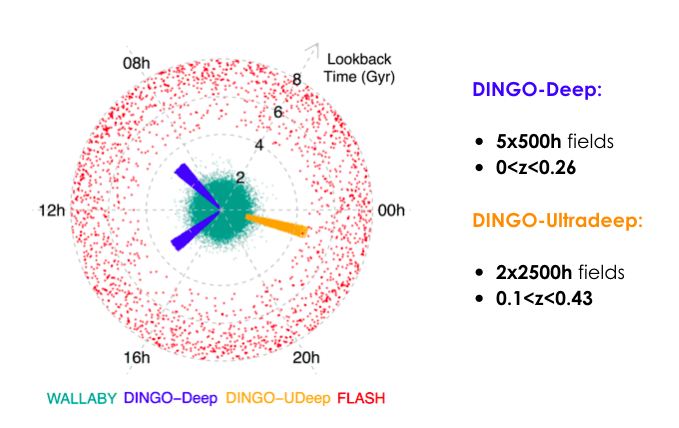
\includegraphics[width=0.75\textwidth]{logos/askap_hi_surveys_meyer.png}
    }
    \caption{Caption of the image is normalsize, balck and no figurenumbering shown by default}
  \end{figure}
\end{frame}


\end{document}
